\section{Phase One: Map Creation}\label{sec:eval_phase1}
To collect measurements for the creation of the map, a person holding a Samsung Galaxy A53 5G phone, with the application described in Section \ref{sec:data_collection_implementation} installed and running, traverses systematically through the room and stops at each collection point to collect measurements for the map. 
We will refer to this person as the \textit{collector}.

During the creation of the map, the collector is responsible for correctly labelling the measurements collected at each collection point shown in Figure \ref{fig:room_partition_measurements}. 
The collector is also responsible for holding the phone in roughly the same heigt when creating the map. 
During this experiment, the collector had the phone out in front of their face when collecting measurements for the map. 
During the map creation, the collector collects measurements for all four beacons until the a standard deviation of under 6.5 xxx insert unit xxx and a minimum of $40$ measurements are established.
This is done by selecting all beacons in the developed application and using the functionality described in Section \ref{sec:first_phase}.

\begin{figure}[h]
    \centering
    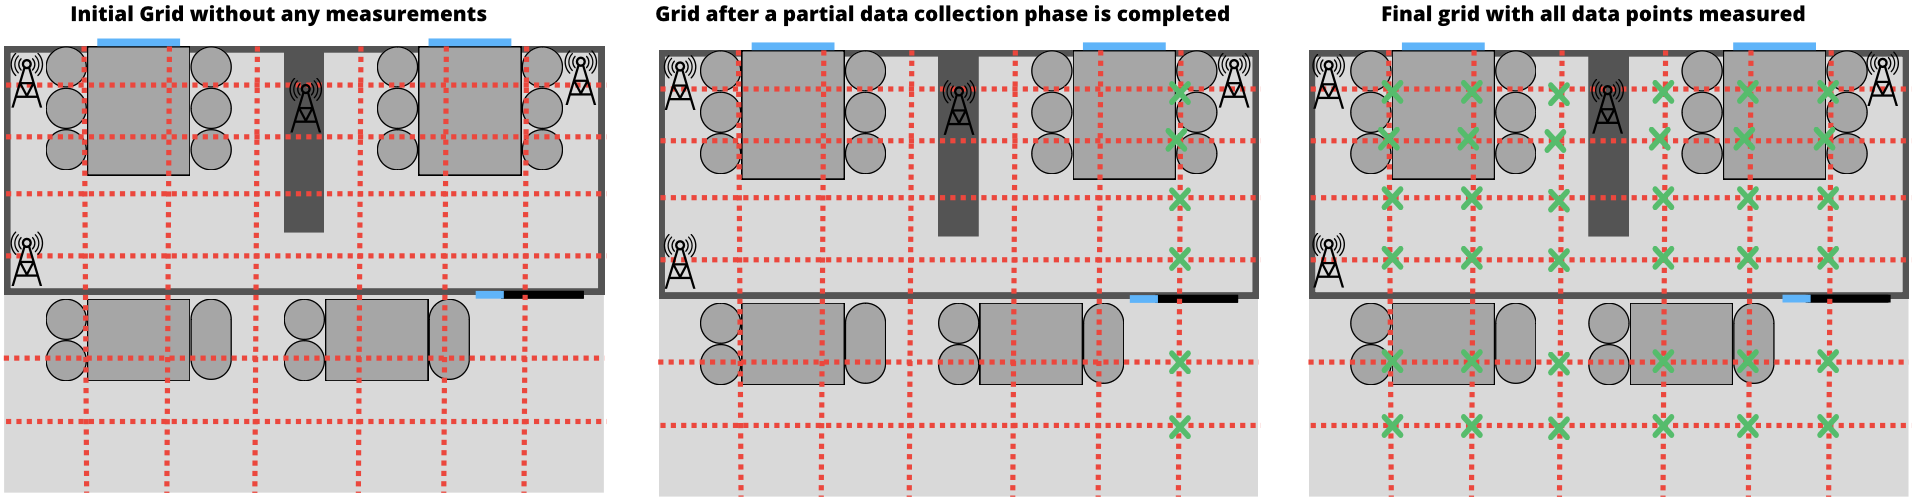
\includegraphics[width=\textwidth]{images/experiment_map_creation.png}
    \caption{A sketch of the meeting room partitioned into a grid decorated with beacon placements (red antenna) and measurement locations (circles with letters). The figure how the measurements are collected systematically in the meeting room.}
    \label{fig:experiment_map_creation}
\end{figure}
Whenever the collector stops at one of the collection points depicted in Figure \ref{fig:room_partition_measurements}, they press a button in the app, which starts measuring after five seconds, as depicted in Figure \ref{fig:collecting_data}.
The phone provides auditory feedback when it has collected enough measurements (in this case 40) and has reached a low enough standard deviation (6.5).
When the information for measurement has been computed and stored on the phone, the collector is informed auditorily and continues to the next intersection in the grid. 
The traversion of the grid is done in systematically, as described in Section \ref{sec:system_overview}. 
Figure \ref{fig:experiment_map_creation} depics a possible systematic traversal starting in the lower right corner of the grid. 


